\documentclass[11pt,a4paper]{article}
\usepackage[margin=2.4cm]{geometry}
\usepackage{graphicx,booktabs,amsmath,amssymb,microtype,xcolor,caption}
\usepackage[hidelinks]{hyperref}
\usepackage{inconsolata}
\usepackage[T1]{fontenc}
\usepackage{lmodern}
\definecolor{ember}{HTML}{FF5A00}
\captionsetup{font=small,labelfont={bf,color=ember}}
\setlength{\parskip}{0.45em}
\setlength{\parindent}{0pt}

\title{\textbf{What does the language actually cost?}\\[.3em]
\large A conformance-verified benchmark of ten TypeScript, Go and Rust
implementations of one database-bound business transaction}
\author{Halleluyah Oludele}
\date{22 September 2026}

\begin{document}
\maketitle

\begin{abstract}
\noindent
Comparisons between server runtimes usually measure microbenchmarks --- JSON
serialisation, a single-row fetch --- and rarely establish that the
implementations being compared do the same work. We specify one composite
business transaction (order pricing and checkout: six reads, a stacking
discount engine, and an eleven-statement write transaction), implement it ten
times across TypeScript, Go and Rust, and verify byte-for-byte output
equivalence across all ten before any timing is recorded. Measuring 450 runs
under pinned CPU sets with a coordinated-omission-safe load generator, we find
that at a fixed 300 requests per second the ten stacks span
1.0~ms of p99 latency, and that Rust and Go are statistically
indistinguishable (0.99$\times$, $p$=0.71). The separations that do survive
correction are between language tiers and, larger than any of them, between
data-access strategies: an ORM costs 1.84$\times$ throughput against the
identical router over hand-written SQL. A zero-dependency Bun service
outperforms both third-party TypeScript stacks. Code, data and analysis are
public.
\end{abstract}

\section{What this measures, and why}

Choosing a backend language is usually argued with throughput numbers drawn
from benchmarks that do very little work per request. The TechEmpower Framework
Benchmarks~\cite{techempower}, the reference point for this comparison, cover
331 frameworks; their database tests fetch one row, or twenty rows, from a
single table. A service that spends most of its time on database round-trips
and application-side business logic is a different regime, and the ranking from
one does not transfer to the other.

Two further gaps motivated this work. First, implementations in a
multi-language benchmark are usually accepted on review rather than proven
equivalent, so a stack can place well by doing marginally less work. Second,
results are typically published as point estimates, with no repetition variance
and no significance testing, which makes it impossible to tell an ordering from
noise.

This is a systems and artifact contribution, not a novel finding: that compiled
languages outperform interpreted ones under saturation is not news. What the
artifact provides is a workload shaped like real business code, a conformance
gate that makes the comparison meaningful, and an analysis that says which
differences are real.

\section{Workload}

The contract is specified once, in \texttt{spec/SPEC.md}, and implemented to the
letter by all ten services. Three endpoints:

\textbf{Pricing (\texttt{POST /api/quote})} issues six reads --- customer joined
to tier, products by SKU, active discount rules, regional tax rates, an optional
coupon, and inventory --- then runs a pure-CPU engine. Each cart line is priced
against every active rule; stacking resolves to the largest non-stackable rule
plus all stackable ones, capped at 60\% of the line; a coupon is spread across
lines pro rata by net value with remainder cents assigned to the largest line;
per-line tax is recomputed on the reduced amount; shipping is banded by total
weight; loyalty points accrue by tier multiplier. All money is integer minor
units and every basis-point multiplication rounds half-up on the final cent, so
the result is exactly reproducible across languages.

\textbf{Checkout (\texttt{POST /api/checkout})} runs the same engine inside one
transaction, taking \texttt{SELECT \ldots FOR UPDATE} on inventory in
product-id order to avoid deadlock, rejecting insufficient stock with HTTP 409,
then writing the order, a multi-row line insert, per-line inventory
reservations, two ledger entries, a coupon usage increment and a loyalty
transaction before committing.

\textbf{Summary (\texttt{GET /api/customers/:id/summary})} performs four reads
over a customer's last 50 orders and their lines and aggregates in process into
lifetime value, top categories by spend, points balance and a segment label.

The dataset holds 50{,}000 customers, 5{,}000 products, 200{,}000 historical
orders and 600{,}247 order lines, generated deterministically from a fixed seed.

\section{Implementations}

\begin{table}[h]\centering\small
\caption{The ten stacks. Within a language the pricing engine is a single
shared module, so framework rows differ only by framework.}
\begin{tabular}{llll}
\toprule
    \textbf{id} & \textbf{Language} & \textbf{Framework} & \textbf{Driver} \\
\midrule
    \texttt{ts-bun-only} & TypeScript & hand-rolled router & Bun.sql (built in, zero deps) \\
    \texttt{ts-bun-hono} & TypeScript & Hono & pg (npm) \\
    \texttt{ts-node-fastify} & TypeScript & Fastify & pg (npm) \\
    \texttt{go-nethttp} & Go & net/http (stdlib) & pgx/v5 \\
    \texttt{go-fiber} & Go & Fiber (fasthttp) & pgx/v5 \\
    \texttt{go-gin} & Go & Gin & pgx/v5 \\
    \texttt{go-gin-gorm} & Go & Gin & GORM \\
    \texttt{rust-hyper} & Rust & hyper (none) & tokio-postgres \\
    \texttt{rust-axum} & Rust & Axum & tokio-postgres \\
    \texttt{rust-actix} & Rust & Actix Web & tokio-postgres \\
\bottomrule
\end{tabular}
\end{table}

Two rows are deliberate exceptions to the shared-module rule.
\texttt{go-gin-gorm} reaches the same logic through an ORM, isolating what the
ORM costs when the router is held constant. \texttt{ts-bun-only} has no
third-party dependency at all: \texttt{Bun.serve} for HTTP, \texttt{Bun.sql} for
Postgres, and a sixty-line router. It runs from a bare directory with no
\texttt{node\_modules} and no lockfile.

\section{Conformance}

Before any measurement, \texttt{bench/verify.py} replays a fixed corpus against
each service in turn and diffs the canonical JSON responses across all ten.
A stack that skipped a query, rounded differently, or computed a different
invoice fails here. Two normalisations are applied: the order id, which is a
database sequence and differs per run, and ISO timestamp spelling, since
\texttt{:00Z} and \texttt{:00.000Z} denote the same instant and the
specification does not dictate fractional-second formatting. All ten
implementations pass.

Conformance establishes that the services return the same bytes, not that they
ask the database the same questions. A second check counts statements reaching
the server under \texttt{log\_statement}: nine services issue 6 statements per
pricing call and 15 per checkout, while \texttt{go-gin-gorm} issues one more of
each, because GORM's \texttt{Preload} resolves the customer tier with a second
\texttt{SELECT} rather than the join the specification prescribes. We report the
divergence rather than remove it: an ORM silently altering the query plan is
part of what the ORM costs, and it accounts for roughly a ninth of its measured
overhead.

\section{Method}

\textbf{Hardware and isolation.} Intel Core i7-8665U (4 cores, 8 threads),
31~GB RAM, Arch Linux 7.1.9. The three parties never share a core: PostgreSQL
18 is confined by Docker to cores 0--2, the service under test by
\texttt{taskset} to 3--5, and the load generator to 6--7. The CPU governor is
pinned to \texttt{performance}; under the default \texttt{powersave} governor an
earlier iteration of this suite showed a 66\% median spread across repetitions.

\textbf{Database.} PostgreSQL 18 in Docker with fixed settings
(\texttt{shared\_buffers=4GB}, \texttt{synchronous\_commit=off},
\texttt{max\_connections=400}). Disabling synchronous commit is a measurement
choice: it removes SSD commit stalls that would otherwise dominate the write
workload. Autovacuum is disabled on the six churned tables and vacuum runs
explicitly between runs; autovacuum firing mid-measurement was the largest
single source of variance we identified. The database is restored to seeded
state before every run.

\textbf{Load generation.} A purpose-built generator runs closed-loop (64
connections, send as fast as the server answers) to find the saturation
ceiling, and open-loop at a fixed arrival rate to measure latency under
controlled load. In open-loop mode latency is measured from each request's
\emph{intended} send time rather than its actual dispatch, which is the
standard correction for coordinated omission: a server that falls behind cannot
hide the delay inside its own slowness. Warmup is excluded from statistics so
JIT-compiled runtimes are not charged for their first requests.

\textbf{Design.} 5 repetitions of 10\,s after 3\,s warmup, across
three workloads and three load profiles, for 450 runs in total. Run order is
shuffled within each repetition so thermal drift cannot systematically favour
whichever stack ran first. Every run records a machine-speed probe --- fixed CPU
work, timed --- so runs taken while the machine was busy remain identifiable;
58 of 450 runs were flagged, and excluding them moves the reported
medians by 0.0\% at the median.

\section{Statistical treatment}

With ten treatments measured over nine tasks (three workloads $\times$ three
load profiles), the appropriate omnibus test is the Friedman
test with Nemenyi post-hoc~\cite{demsar}, whose power derives from the number of
tasks rather than the number of repetitions, and which assumes no error
distribution. We report medians and bootstrap intervals for transparency but
base significance claims on the rank-based tests.

Friedman rejects the null for p99 latency ($\chi^2$=56.7, $p$=5.8e-09), for CPU
per request ($\chi^2$=77.4, $p$=5.2e-13) and for peak memory
($\chi^2$=80.6, $p$=1.2e-13), each over $N$=9 tasks and $k$=10 treatments. The
Nemenyi critical difference at the 5\% level is 4.52 ranks.

Five pairwise contrasts were specified before data collection, each
corresponding to one design question. For these, throughput is normalised
within each workload by that workload's grand median across stacks and pooled,
giving 15 independent runs per stack; they are compared with the Mann--Whitney
$U$ test under Holm correction across the family of five. Normalising within
workload is what makes pooling legitimate --- the three workloads differ by
almost an order of magnitude in absolute throughput --- and the power comes from
blocking, not from re-using observations.

\section{Results}

\begin{figure}[h]\centering
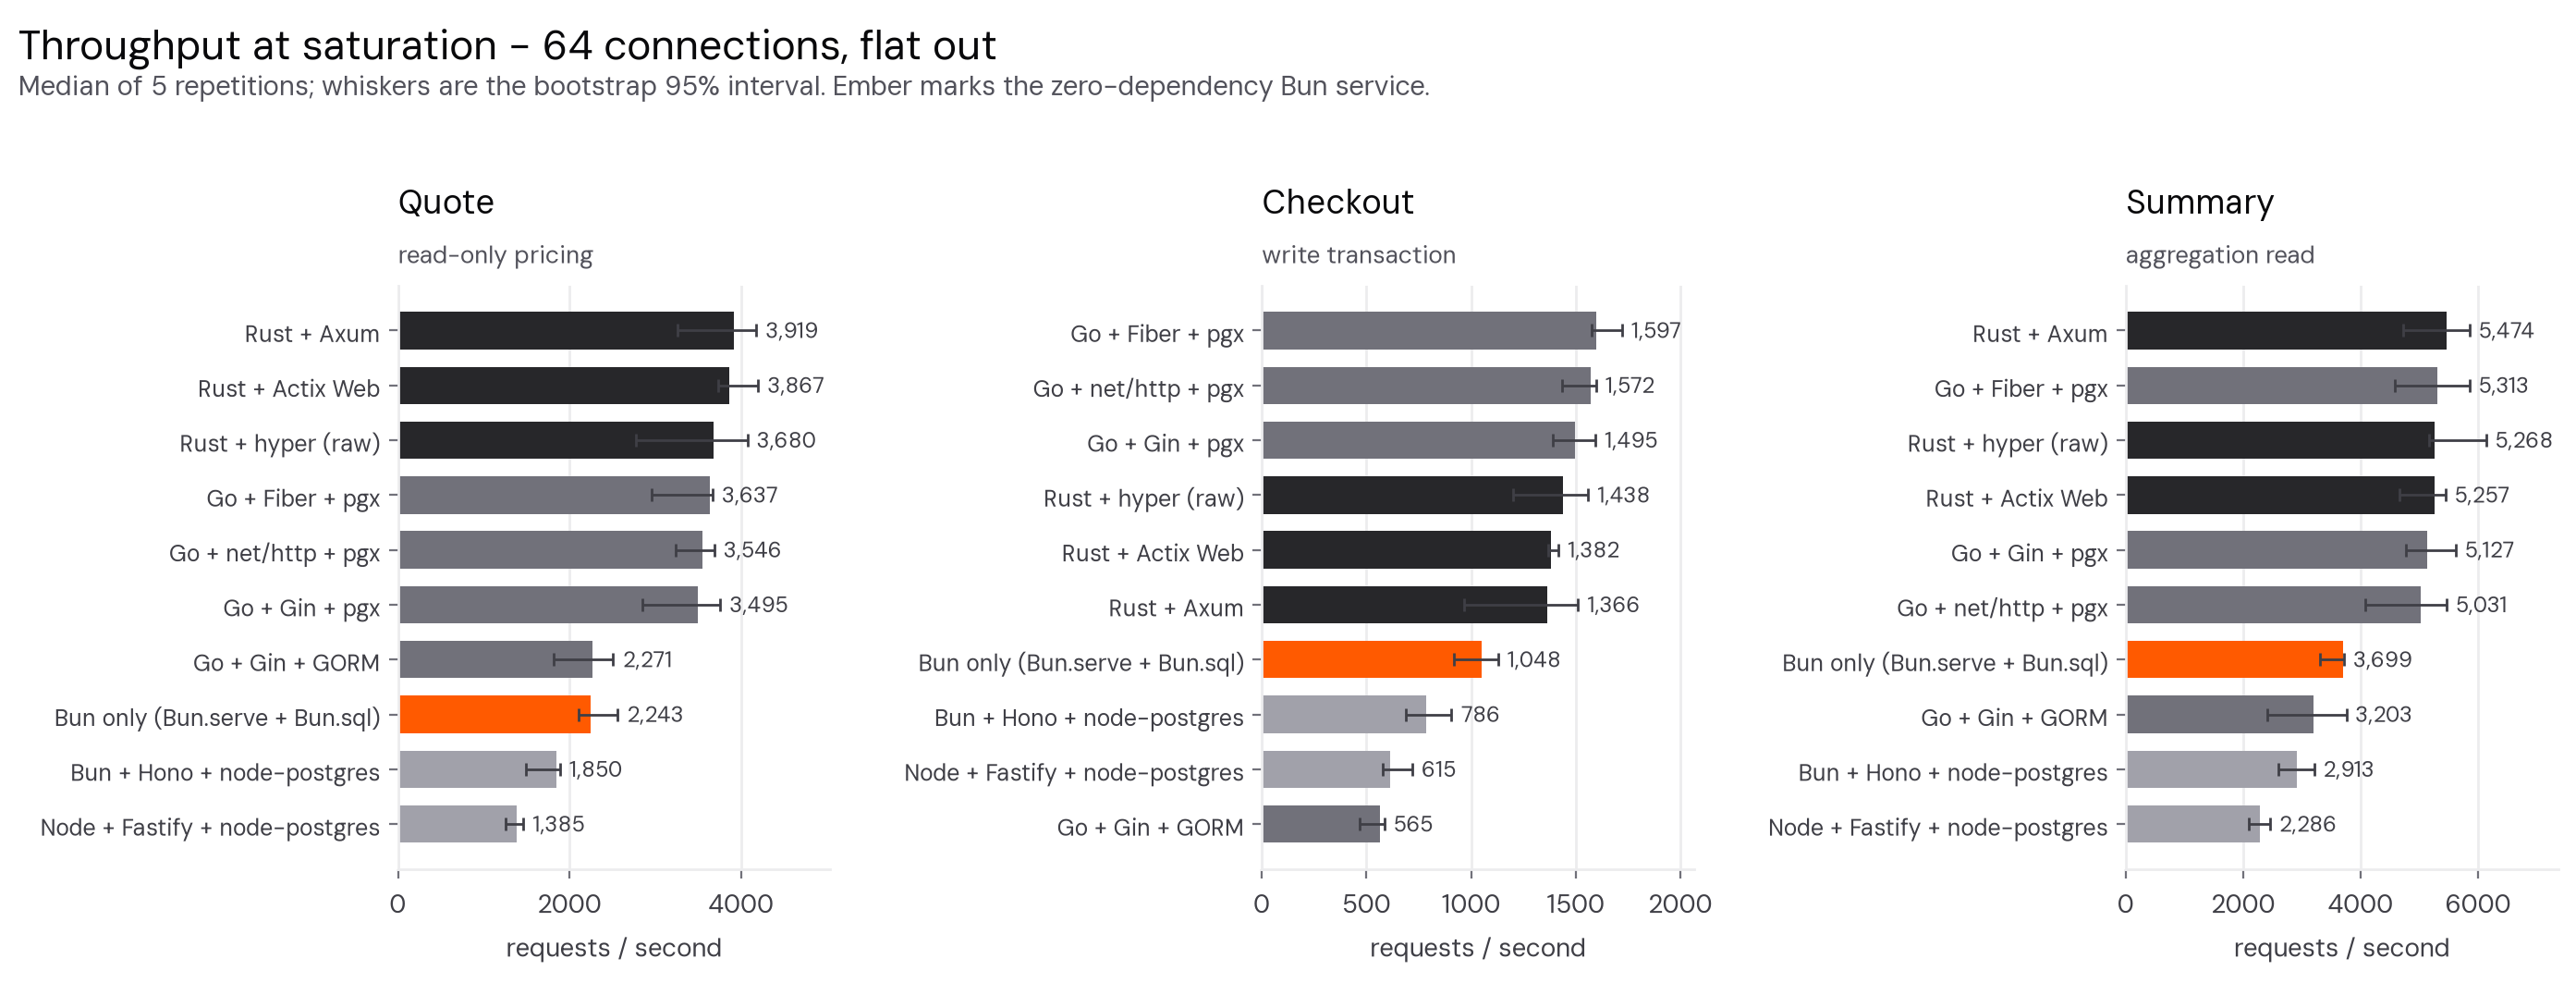
\includegraphics[width=\textwidth]{../docs/figures/throughput.png}
\caption{Throughput at saturation. Whiskers are bootstrap 95\% intervals over
5 repetitions.}
\end{figure}

\subsection{Under realistic load, the runtime is not the variable}

At a fixed 300 requests per second the ten stacks span 1.0~ms of p99
latency, from 2.64~ms (\texttt{go-nethttp}) to 3.60~ms (\texttt{ts-bun-hono}).
Figure~\ref{fig:load} shows that the spread only opens as offered load
approaches each stack's ceiling.

\begin{figure}[h]\centering
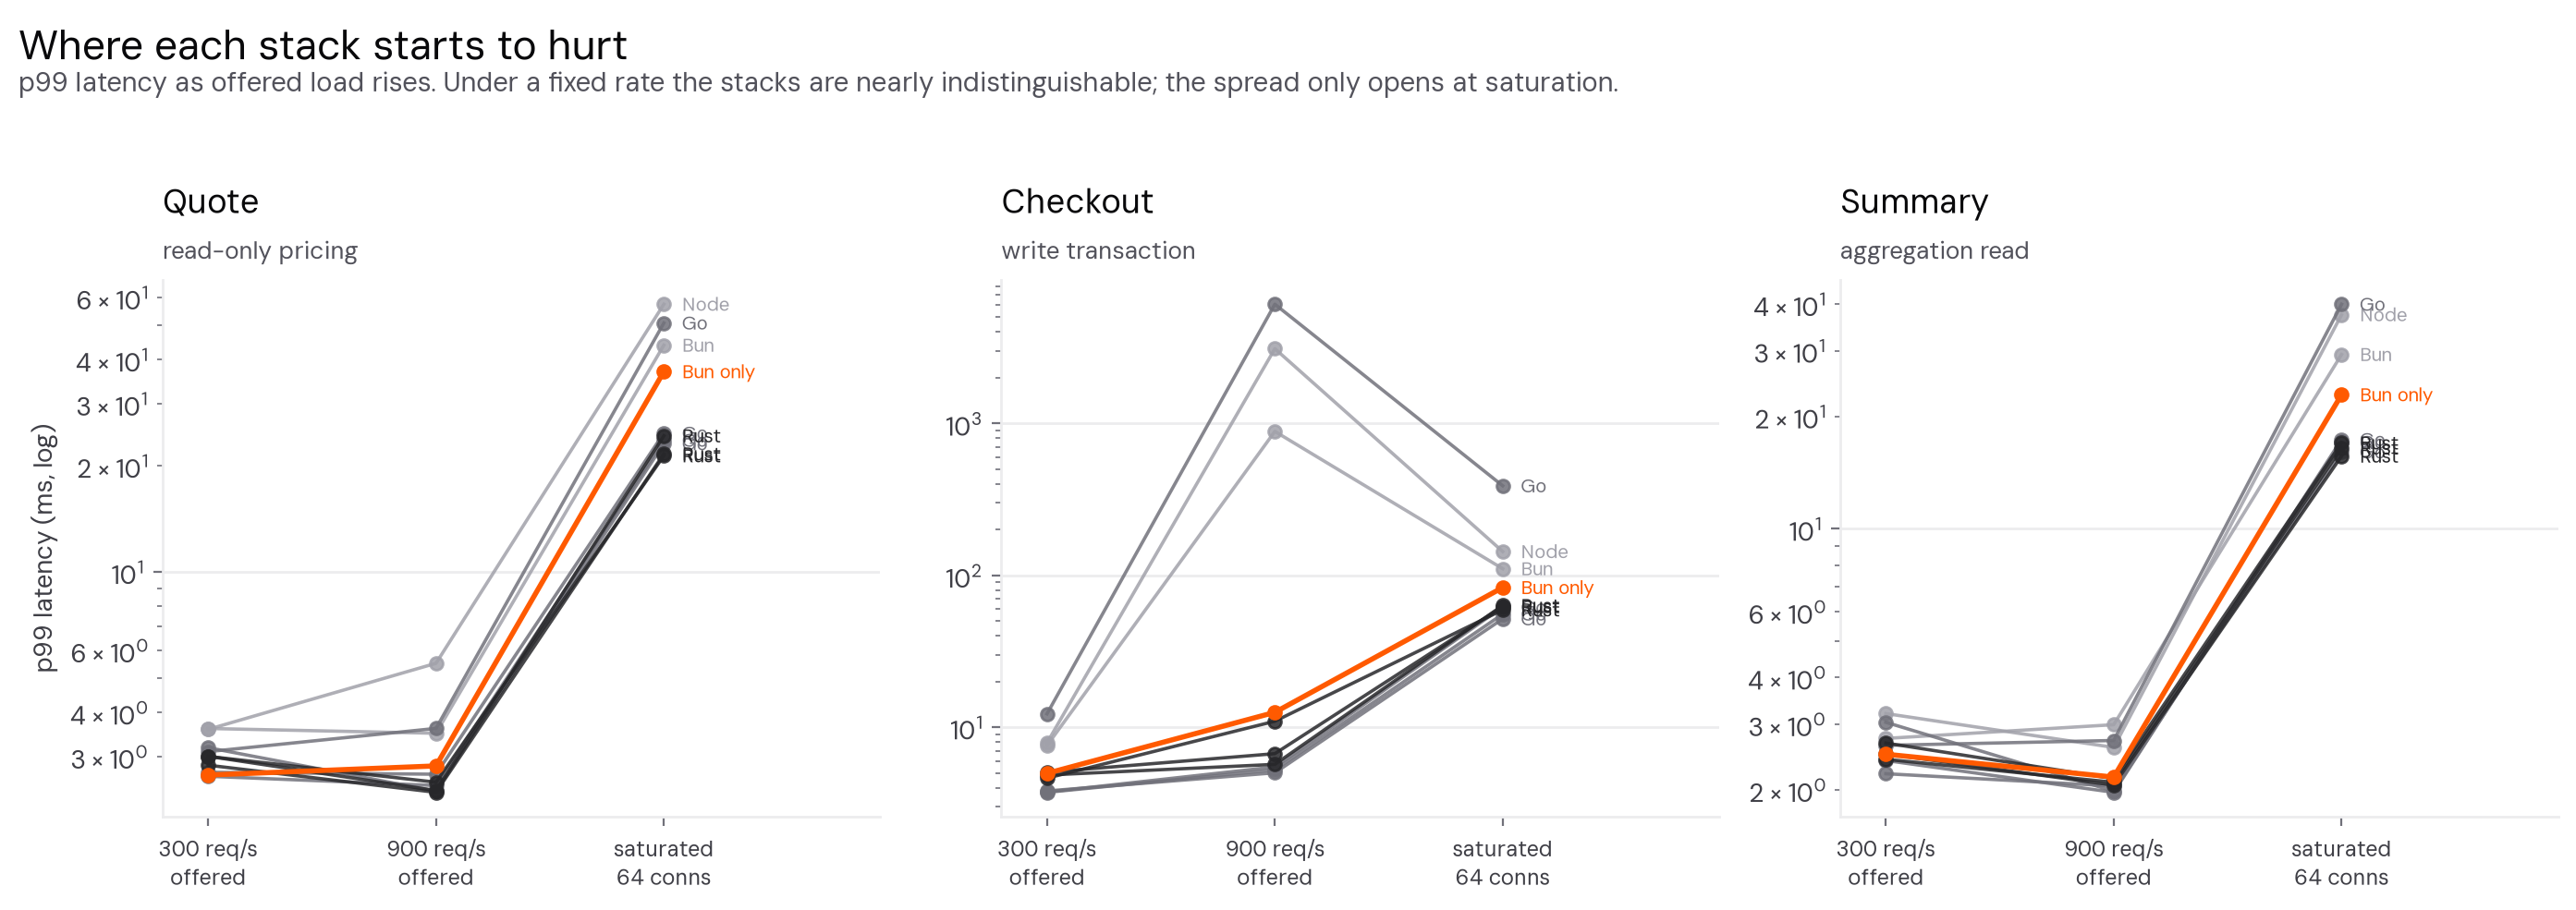
\includegraphics[width=\textwidth]{../docs/figures/latency_vs_load.png}
\caption{p99 latency as offered load rises.}\label{fig:load}
\end{figure}

\begin{table}[h]\centering\small
\caption{Saturated throughput (req/s) and p99 (ms) per workload; CPU
milliseconds per request and peak resident memory are for the pricing
workload.}
\begin{tabular}{lrrrrrrrr}
\toprule
 & \multicolumn{2}{c}{Quote} & \multicolumn{2}{c}{Checkout}
 & \multicolumn{2}{c}{Summary} & CPU & RSS \\
\cmidrule(lr){2-3}\cmidrule(lr){4-5}\cmidrule(lr){6-7}
    \textbf{stack} & req/s & p99 & req/s & p99 & req/s & p99 & ms & MB \\
\midrule
    \texttt{rust-axum} & 3,919 & 21.6 & 1,366 & 63.5 & 5,474 & 15.7 & 0.281 & 8 \\
    \texttt{rust-actix} & 3,867 & 21.4 & 1,382 & 62.4 & 5,257 & 17.0 & 0.317 & 9 \\
    \texttt{rust-hyper} & 3,680 & 24.3 & 1,438 & 59.4 & 5,268 & 16.5 & 0.271 & 8 \\
    \texttt{go-fiber} & 3,637 & 23.1 & 1,597 & 51.8 & 5,313 & 16.1 & 0.409 & 22 \\
    \texttt{go-nethttp} & 3,546 & 23.6 & 1,572 & 55.7 & 5,031 & 17.4 & 0.444 & 23 \\
    \texttt{go-gin} & 3,495 & 24.8 & 1,495 & 62.0 & 5,127 & 17.1 & 0.457 & 31 \\
    \texttt{go-gin-gorm} & 2,271 & 50.8 & 565 & 389.1 & 3,203 & 40.0 & 1.125 & 35 \\
    \bfseries \texttt{ts-bun-only} & 2,243 & 37.0 & 1,048 & 83.3 & 3,699 & 22.9 & 0.401 & 79 \\
    \texttt{ts-bun-hono} & 1,850 & 44.0 & 786 & 110.8 & 2,913 & 29.3 & 0.518 & 92 \\
    \texttt{ts-node-fastify} & 1,385 & 57.4 & 615 & 143.6 & 2,286 & 37.5 & 0.730 & 243 \\
\bottomrule
\end{tabular}
\end{table}

\subsection{Rank analysis}

\begin{figure}[h]\centering
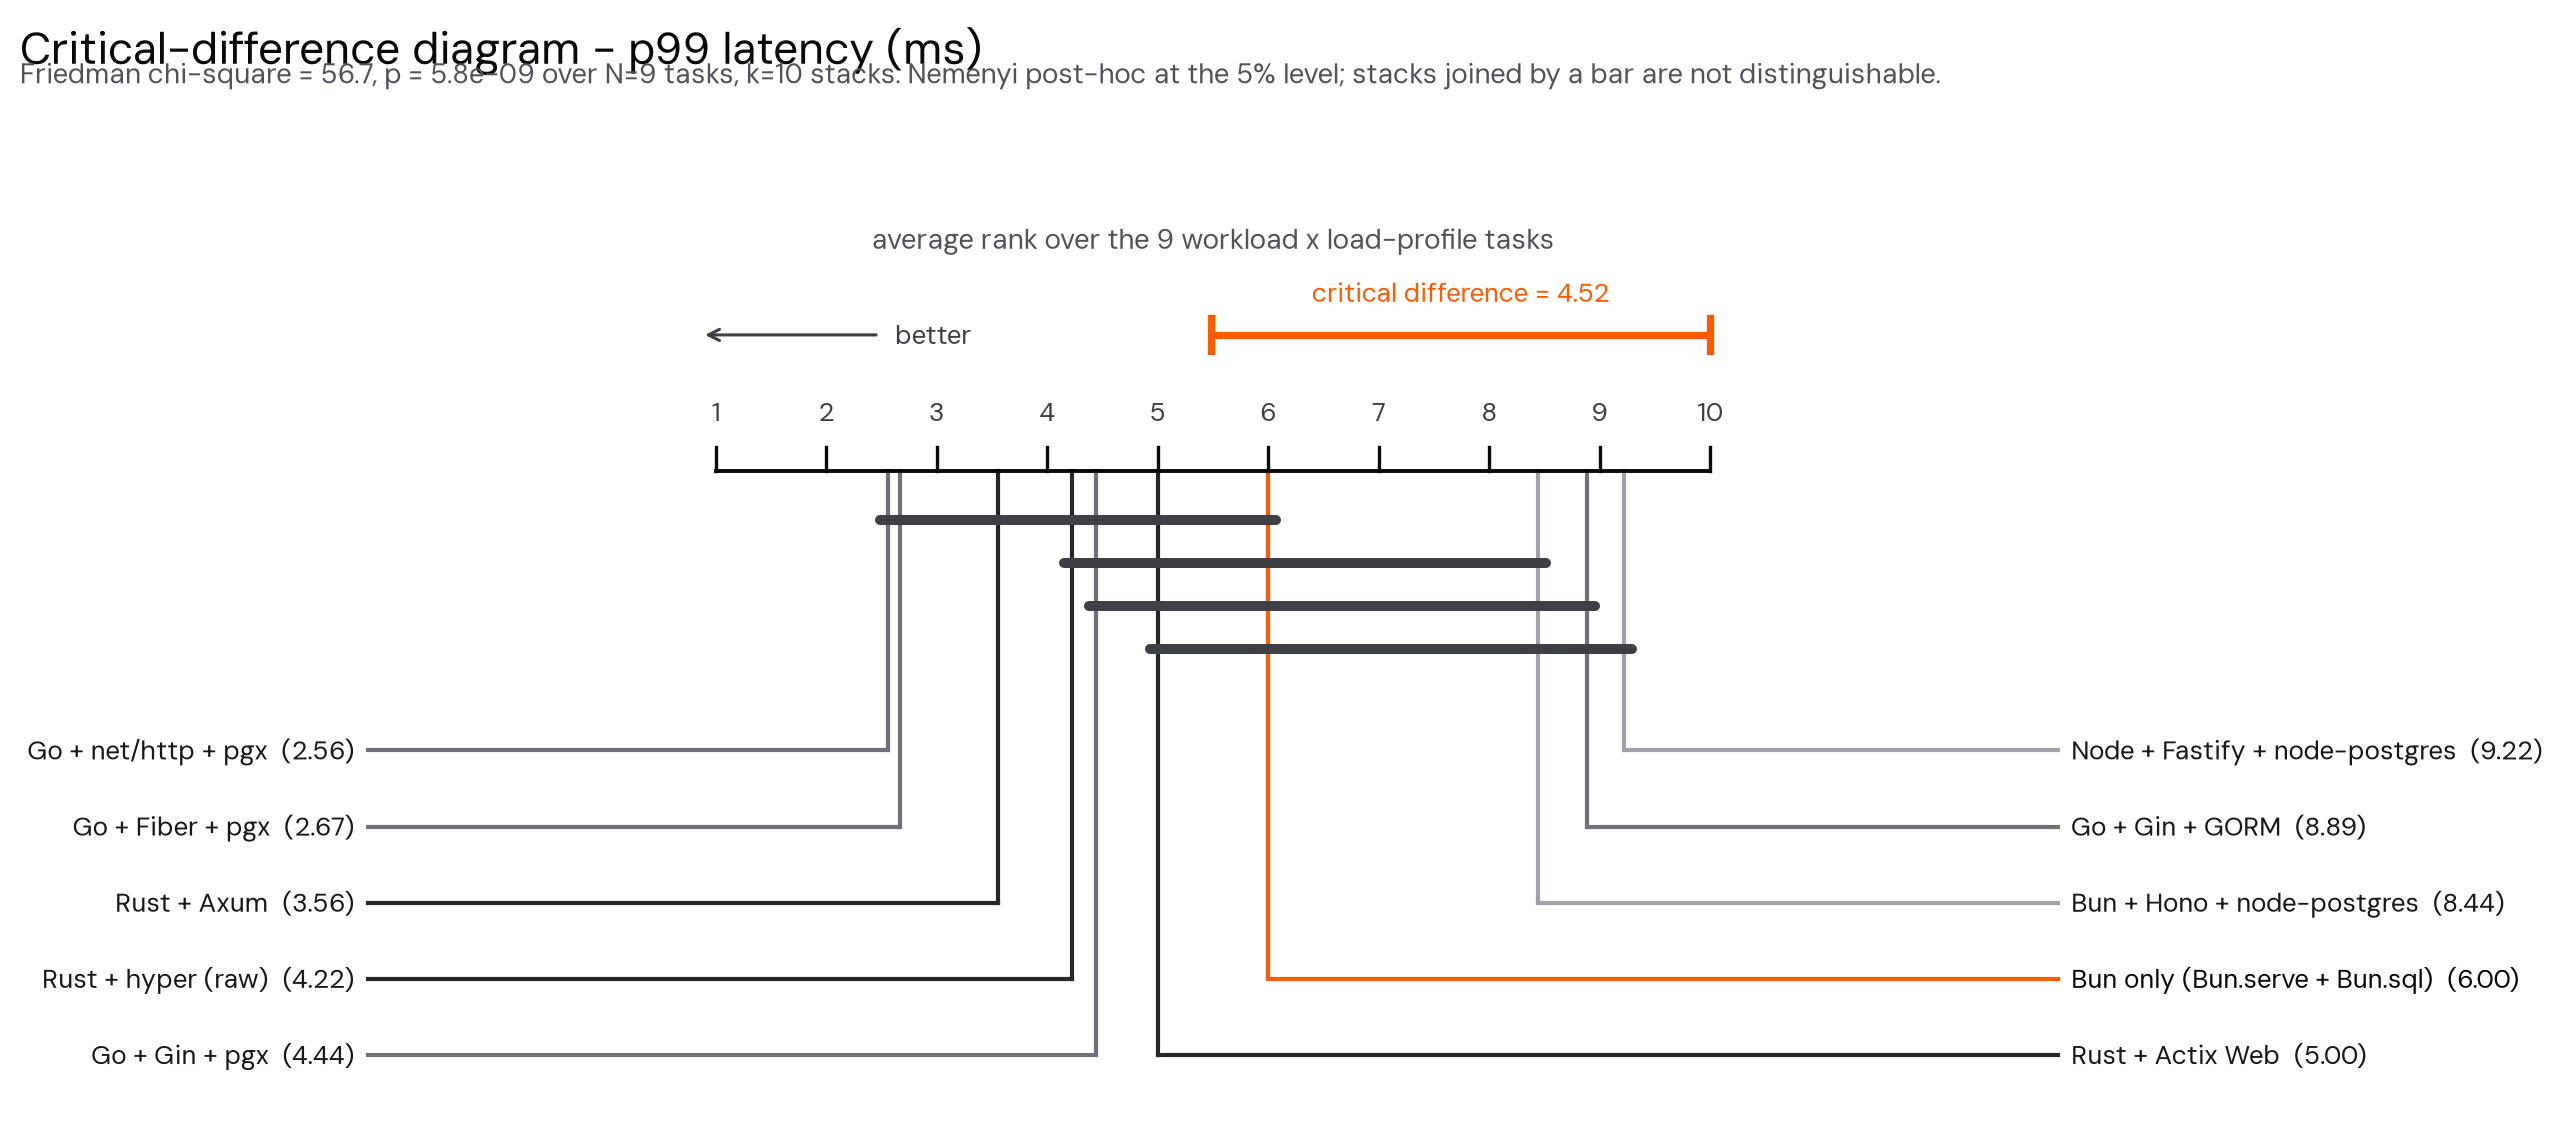
\includegraphics[width=\textwidth]{../docs/figures/cd_p99.png}
\caption{Critical-difference diagram for p99 latency. Stacks joined by a bar
are not distinguishable at the 5\% level.}
\end{figure}

\begin{table}[h]\centering\small
\caption{Average Friedman ranks over the nine tasks (1 = best).}
\begin{tabular}{lr@{\hskip 2.2em}lr}
\toprule
\multicolumn{2}{c}{\textbf{p99 latency}} & \multicolumn{2}{c}{\textbf{CPU per request}} \\
\cmidrule(lr){1-2}\cmidrule(lr){3-4}
    stack & rank & stack & rank \\
\midrule
    \texttt{go-nethttp} & 2.56 & \texttt{rust-hyper} & 1.22 \\
    \texttt{go-fiber} & 2.67 & \texttt{rust-axum} & 1.78 \\
    \texttt{rust-axum} & 3.56 & \texttt{rust-actix} & 3.22 \\
    \texttt{rust-hyper} & 4.22 & \texttt{go-fiber} & 3.89 \\
    \texttt{go-gin} & 4.44 & \texttt{go-nethttp} & 5.39 \\
    \texttt{rust-actix} & 5.00 & \texttt{go-gin} & 6.39 \\
    \texttt{ts-bun-only} & 6.00 & \texttt{ts-bun-only} & 6.44 \\
    \texttt{ts-bun-hono} & 8.44 & \texttt{ts-bun-hono} & 7.67 \\
    \texttt{go-gin-gorm} & 8.89 & \texttt{ts-node-fastify} & 9.00 \\
    \texttt{ts-node-fastify} & 9.22 & \texttt{go-gin-gorm} & 10.00 \\
\bottomrule
\end{tabular}
\end{table}

\subsection{Planned contrasts}

\begin{table}[h]\centering\small
\caption{Pre-specified contrasts on saturated throughput. Ratios above one
favour the first stack; intervals are bootstrap 95\%.}
\begin{tabular}{llrrrc}
\toprule
    \textbf{contrast} & \textbf{question} & \textbf{ratio} & \textbf{95\% CI}
    & \textbf{$p$ (Holm)} & \textbf{sig.} \\
\midrule
    \texttt{ts-bun-only} vs \texttt{ts-node-fastify} & Bun vs Node, both TypeScript & 1.72 & [1.51, 1.83] & 1.7e-05 & \checkmark \\
    \texttt{go-gin} vs \texttt{go-gin-gorm} & Cost of the ORM, router held constant & 1.84 & [1.54, 2.56] & 1.7e-05 & \checkmark \\
    \texttt{ts-bun-only} vs \texttt{ts-bun-hono} & Zero-dependency Bun vs Hono + node-postgres & 1.33 & [1.18, 1.42] & 2.2e-05 & \checkmark \\
    \texttt{rust-axum} vs \texttt{ts-bun-only} & Best Rust vs best TypeScript & 1.45 & [1.30, 1.64] & 4.7e-05 & \checkmark \\
    \texttt{rust-axum} vs \texttt{go-fiber} & Best Rust vs best Go & 0.99 & [0.86, 1.07] & 7.1e-01 & -- \\
\bottomrule
\end{tabular}
\end{table}

\begin{figure}[h]\centering
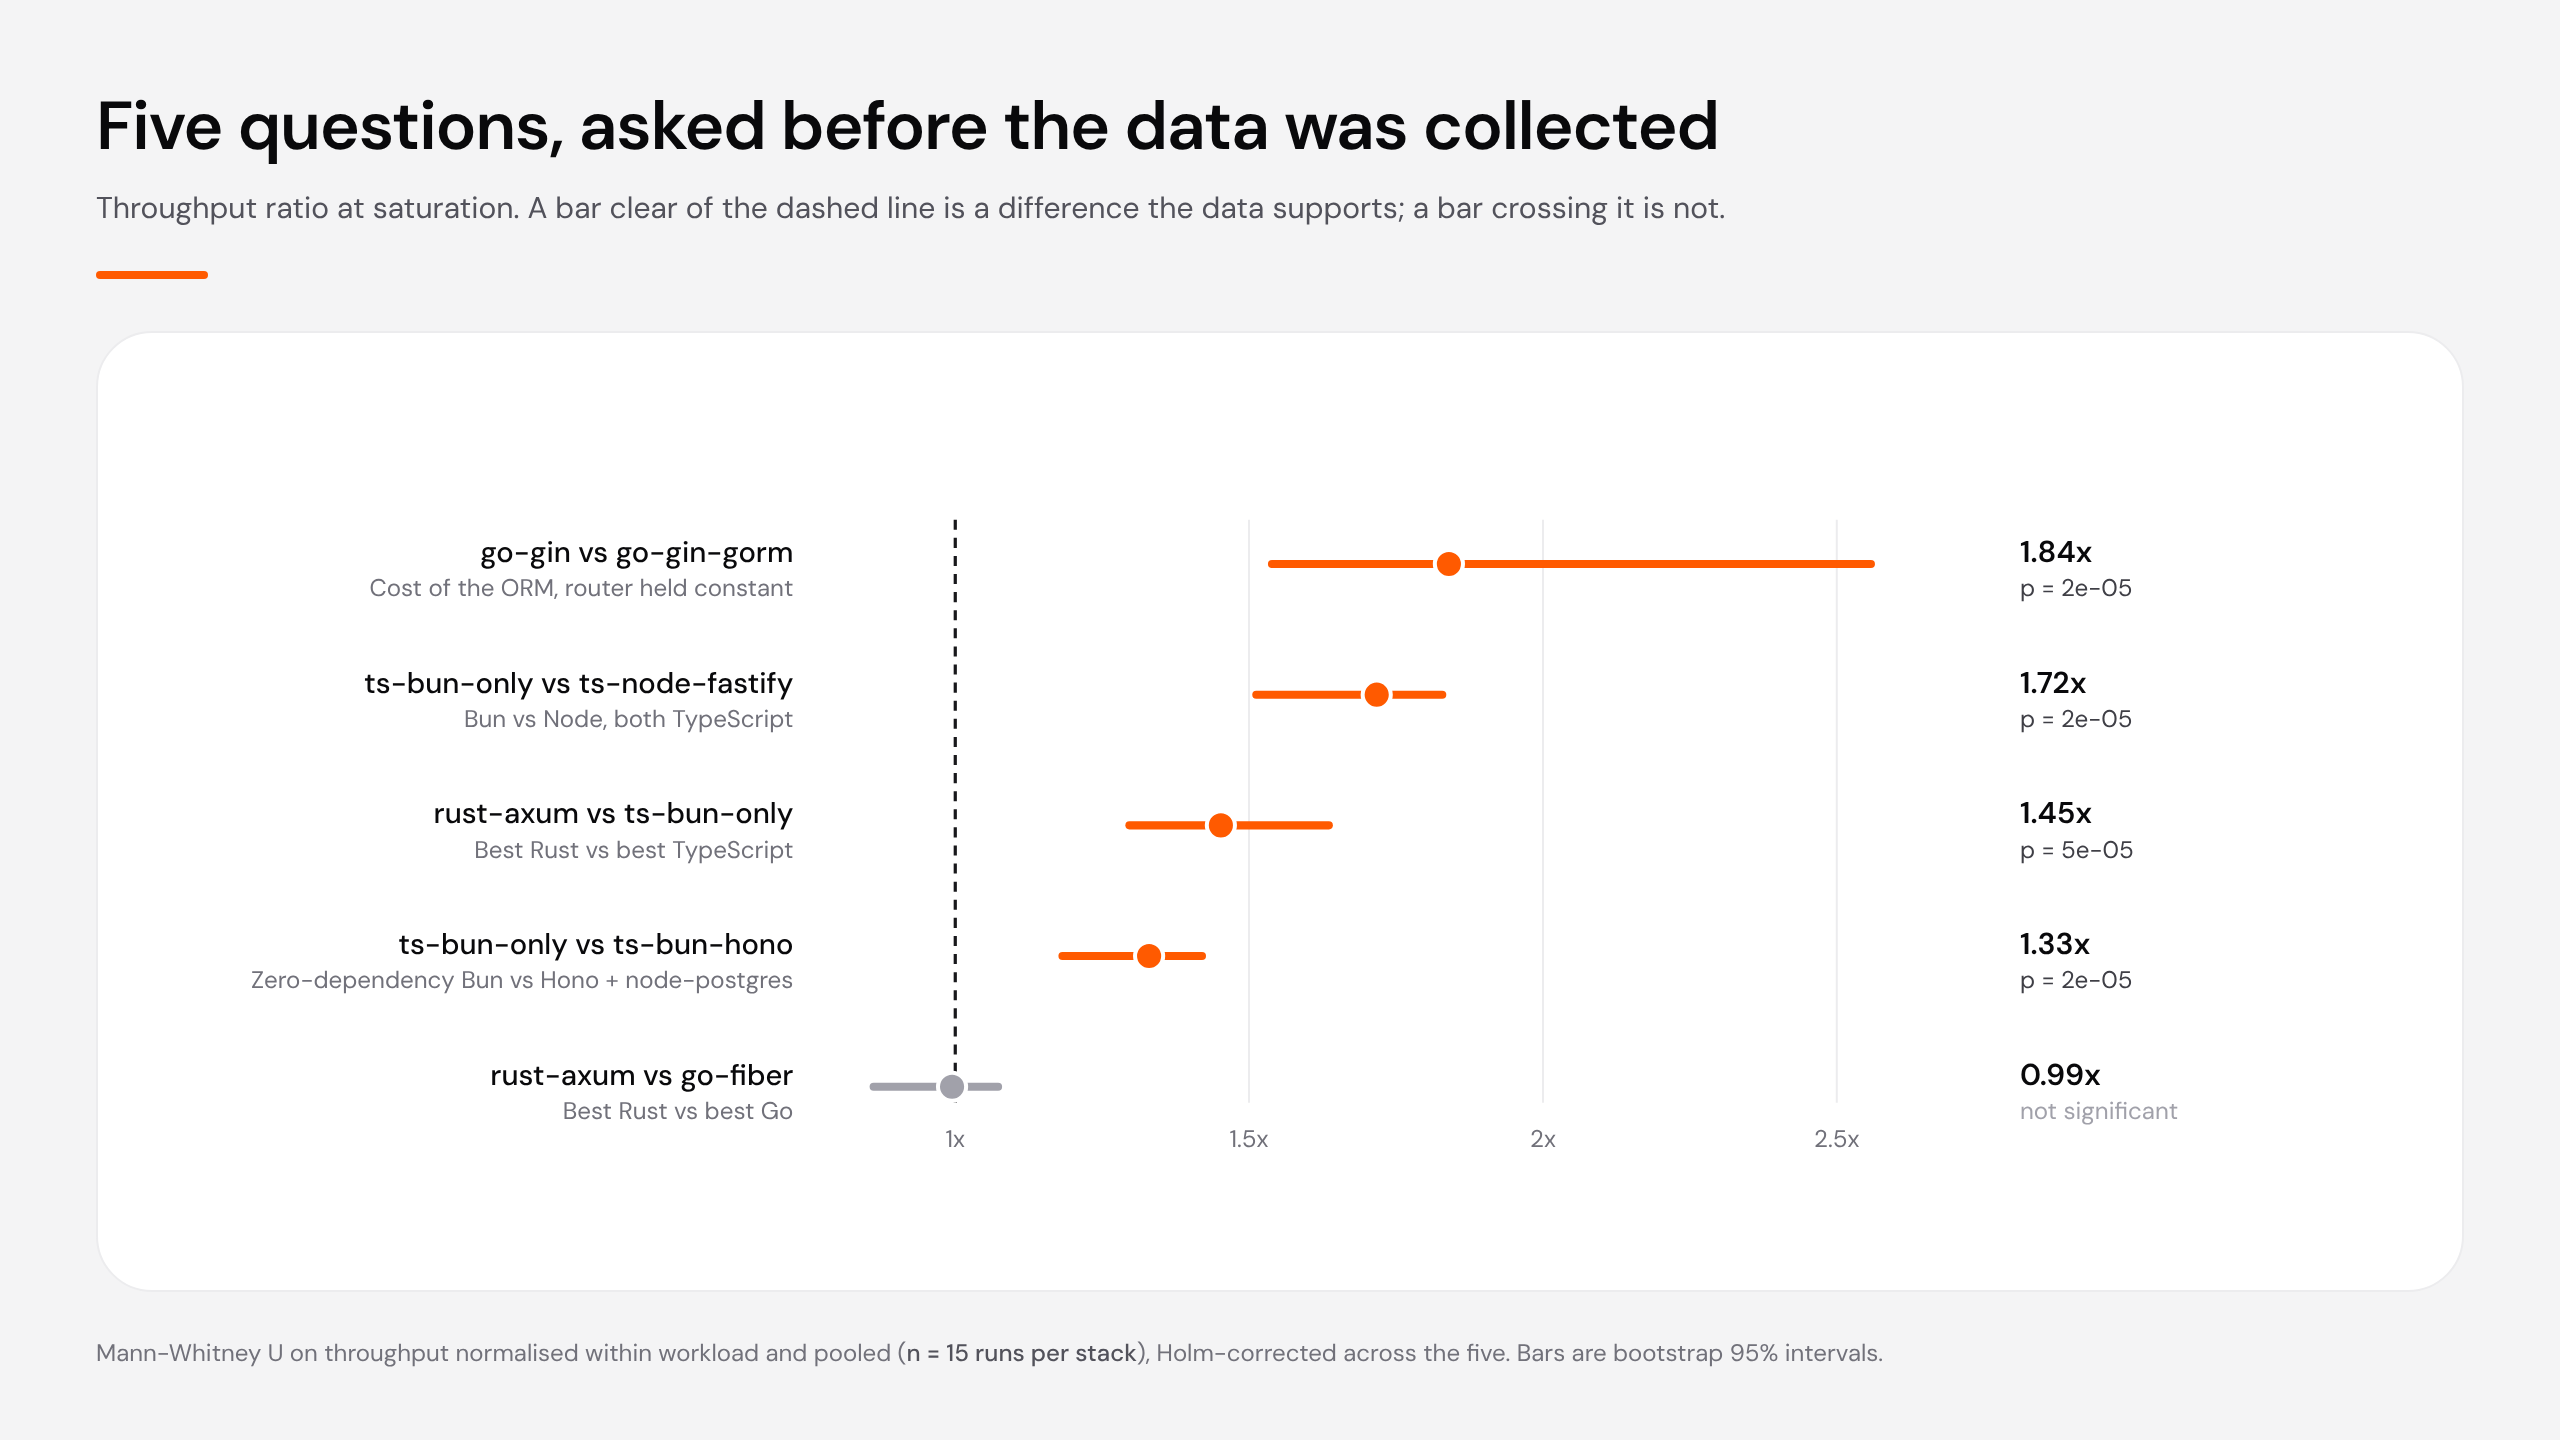
\includegraphics[width=\textwidth]{../docs/figures/contrasts.png}
\caption{The five planned contrasts.}
\end{figure}

Three findings survive correction. \textbf{Rust and Go are indistinguishable on
this workload}: \texttt{rust-axum} against \texttt{go-fiber} gives
0.99$\times$ (95\% CI [0.86, 1.07], $p$=0.71). \textbf{The zero-dependency Bun
service outperforms both third-party TypeScript stacks}, by 1.33$\times$
against Hono with node-postgres and 1.72$\times$ against Node with Fastify.
\textbf{The ORM is the single largest cost on the board}: holding the Gin router
constant and changing only the data layer gives 1.84$\times$ throughput, and
on the write workload GORM consumes 2.87~ms of CPU per request against
0.83~ms.

\begin{figure}[h]\centering
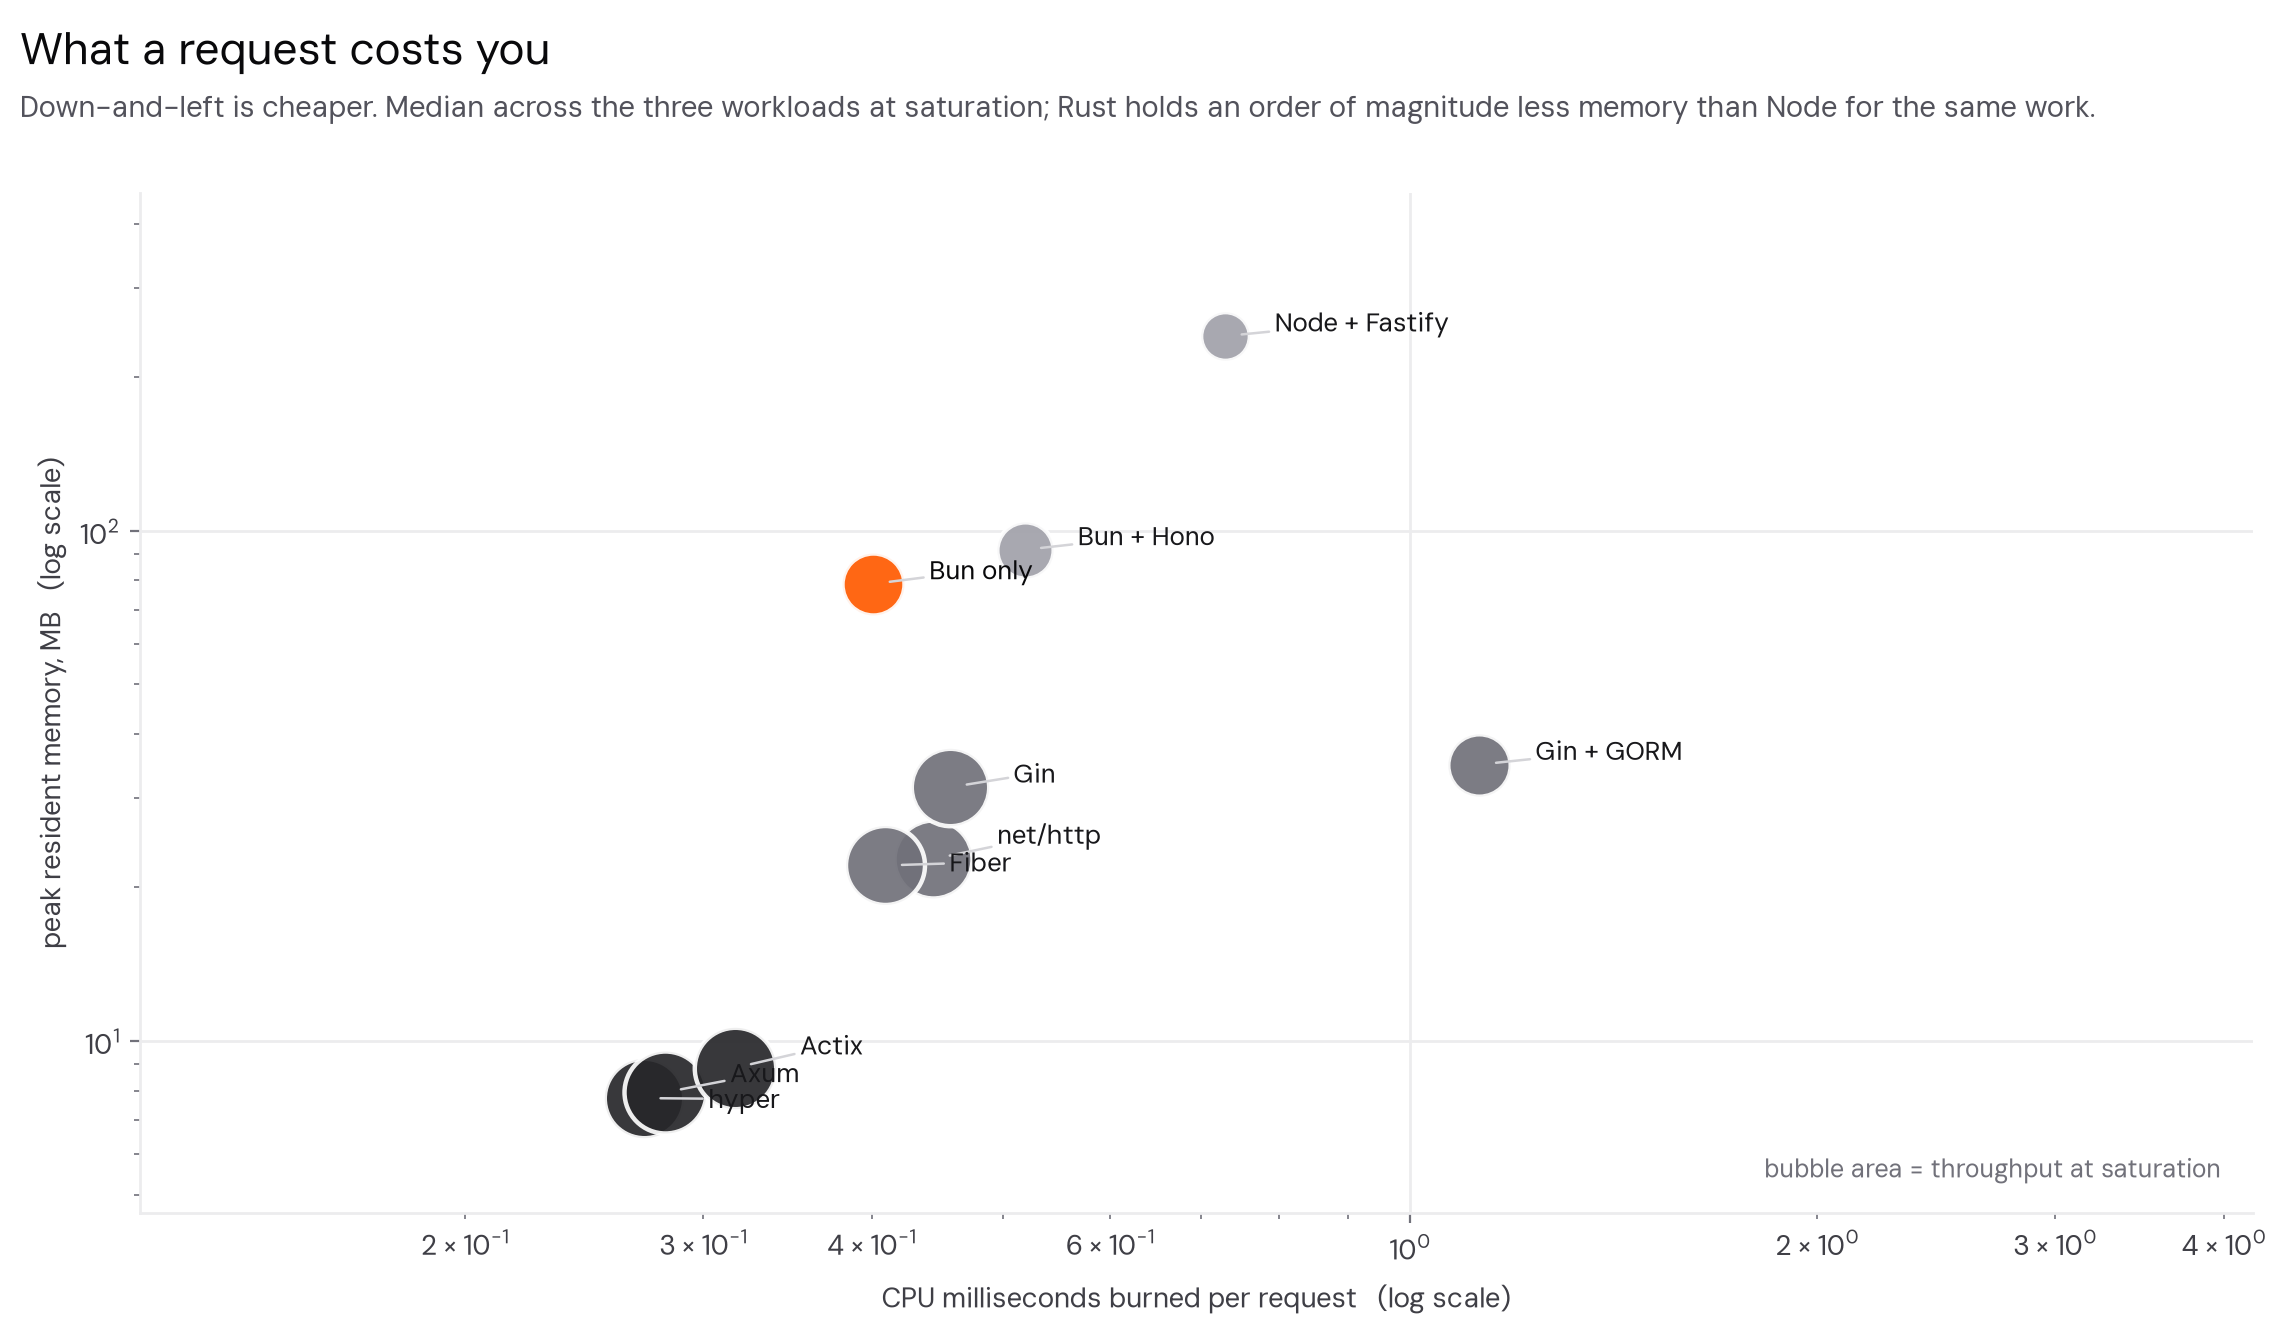
\includegraphics[width=.94\textwidth]{../docs/figures/cost_of_request.png}
\caption{CPU and memory cost per request; bubble area is saturated throughput.}
\end{figure}

\section{Limitations}

One machine, one database, loopback networking, one shape of workload. A
four-core laptop is not a server, and the database sharing a socket with
everything else compresses gaps that a larger machine would widen. The ratios
describe how these stacks handle a database-bound transactional API on this
hardware; the absolute numbers belong to this machine.

Nothing here speaks to streaming, CPU-bound compute, cold-start behaviour, or
performance across a real network.

The ordering \emph{within} a language is not a result. Rust's hyper, Axum and
Actix fall inside the critical difference of one another, as do Go's Fiber,
net/http and Gin; they change places depending on which repetitions are
included. The language tiers are robust, the intra-tier ranking is not.

Five repetitions per cell is few. The intervals quoted are percentile bootstrap
intervals on a median of five: an honest width, not a precise coverage
guarantee. An earlier iteration of this suite with three repetitions and no
machine-speed probe produced a 66\% median spread across repetitions, and the
ranking it implied was partly an artifact of autovacuum and of unpinned
neighbouring processes. That failure is the reason the probe exists.

\section{Future work}

A second machine class would separate hardware-specific effects from stack
effects. Adding Hono over \texttt{Bun.sql} would disentangle router cost from
driver cost in the TypeScript tier, which the present design confounds. Running
the database on a separate host would restore the network round-trip that this
loopback setup removes.

\section{Availability}

Source, raw per-run results, analysis scripts and the generator for every figure
in this report are at \url{https://github.com/hallelx2/polyglot-bench} under the
MIT licence. Every number here is produced by \texttt{analysis/stats.py} from
the run files; none is transcribed by hand.

\begin{thebibliography}{9}
\bibitem{techempower} TechEmpower.
\emph{Framework Benchmarks, Round 23}, March 2025.
\url{https://www.techempower.com/benchmarks/}
\bibitem{demsar} J. Dem\v{s}ar.
\emph{Statistical Comparisons of Classifiers over Multiple Data Sets.}
Journal of Machine Learning Research, 7:1--30, 2006.
\end{thebibliography}

\end{document}
